\documentclass[11pt, oneside]{article}   	% use "amsart" instead of "article" for AMSLaTeX format
\usepackage{geometry}                		% See geometry.pdf to learn the layout options. There are lots.
\geometry{letterpaper}                   		% ... or a4paper or a5paper or ... 
%\geometry{landscape}                		% Activate for for rotated page geometry
%\usepackage[parfill]{parskip}    		% Activate to begin paragraphs with an empty line rather than an indent
\usepackage{graphicx}				% Use pdf, png, jpg, or eps§ with pdflatex; use eps in DVI mode
								% TeX will automatically convert eps --> pdf in pdflatex		
\usepackage{amssymb}
\usepackage{amsmath}
\usepackage{gensymb}				% degree symbol
\usepackage{amsthm}
\usepackage{booktabs}				% allows toprule and bottomrule in tables
\usepackage{tabularx}
\usepackage{multirow}				% data spans multiple rows and columns in tables
\usepackage[makeroom]{cancel}		% e.g. \cancelto{\infty}{5y}
\usepackage{caption}
\usepackage{setspace}

\providecommand{\e}[1]{\ensuremath{\times 10^{#1}}} 		% Scientific notation, e.g.: 6.653 \e{-24}


\usepackage{lscape}

\usepackage{fancyheadings}			% customizable headers and footers
\usepackage{lastpage}
\pagestyle{fancy}
\lhead{}
\chead{}
\rhead{}
\lfoot{}
\cfoot{}
\rfoot{\thepage \, of \pageref{LastPage}}

\makeatletter         
\def\@maketitle{   					% custom maketitle 
\begin{center} \Large \bfseries \@title \end{center}
\begin{flushleft} \@author \\ \@date \end{flushleft} \par 
\smallskip \hrule}

\setcounter{secnumdepth}{0}                     % Only number sections, nothing deeper

\title{Lab 6: Shielding Design for a Co-60 Vault \\ } 
\author{Author: John Hayes \\ Group 1: A. Roth, M. Batie, C. Hoffman, G. Zhao, J. Beres, R. Shirley \\ Course: MP 569 \\ Lab No.: 6 \\ Performed: Wed 4/29/15 }
\date{Due: Wed 5/13/15}							% Activate to display a given date or no date

\begin{document}
\maketitle
\doublespacing
%
\section{Abstract} 

Shielding designs for two walls in a Co-60 vault are determined.  The exposure rate was 2458 R/hr at 1 m from the source, which equates to a workload of the beam of 492 Gy/wk.  

\clearpage
\section{Theory}

Shielding of radioactive sources in any facility that houses them is required to protect personnel and the general public.  
%
\begin{subequations} \label{eqn:Pvalues}
\begin{align} 
P_c &= 5 \, \text{mSv/yr} = 0.1 \, \text{mSv/wk}  \\
P_u &= 1 \, \text{mSv/yr} = 0.02 \, \text{mSv/wk}.
\end{align} 
\end{subequations}
%
The weekly rate is based on fifty 5-day workweeks (allowing for 10 days of holiday.)    As the data section will show, 
%
\begin{equation} \label{eqn:numTVL}
n = -\log(B_T)
\end{equation}
%
Finally, a schematic of the UWMRRC Co-60 vault is shown in Fig \ref{fig:UWMRRC}. 
%
\begin{figure}[h]
    \centering
    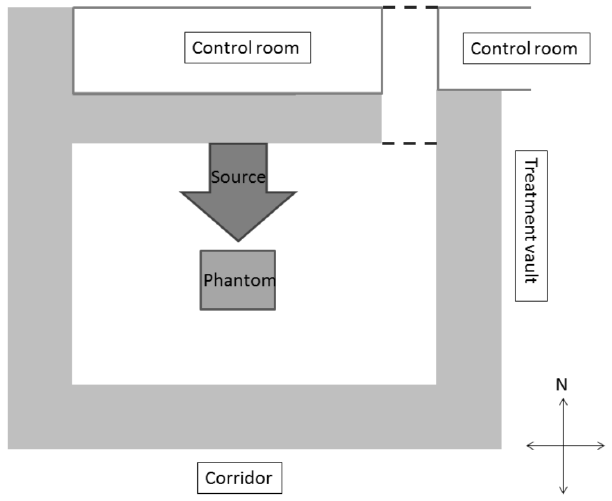
\includegraphics[scale=0.6]{UWMRRC.png}
        \caption{Schematic of the UWMRRC Co-60 vault.}
    \label{fig:UWMRRC}
\end{figure}

\clearpage
\section{Data}

\begin{figure}[h!]
    \centering
    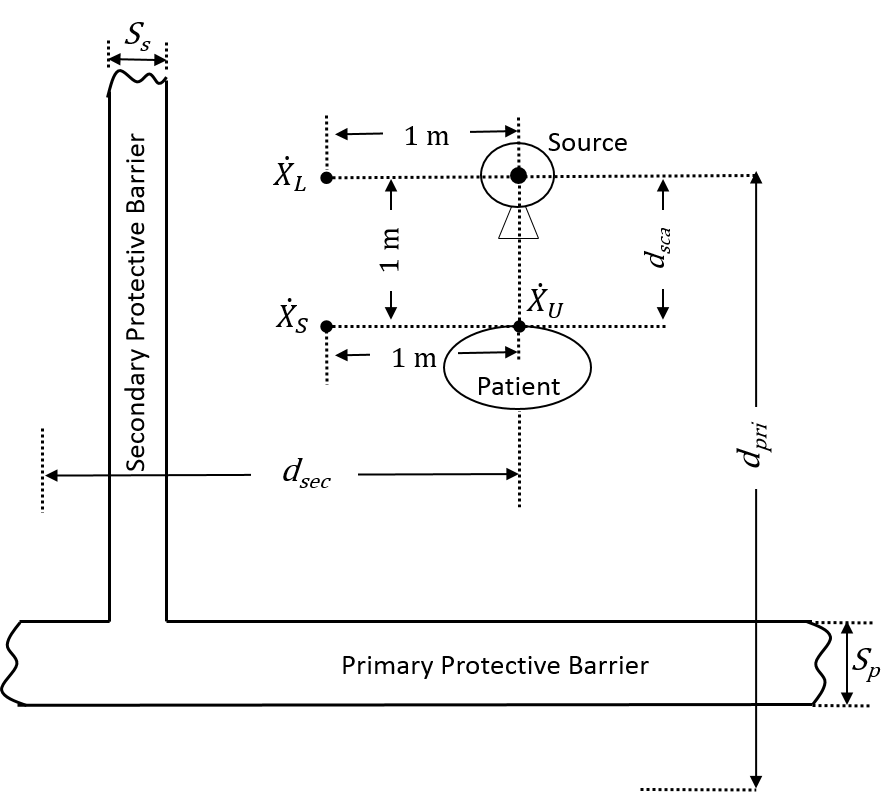
\includegraphics[scale=0.6]{shieldingParams.png}
        \caption{Schematic of parameters required in shielding calculations.}
    \label{fig:shieldingParams}
\end{figure}

%%%%%%%%%%%%%%%%%
\begin{table}[h!]
\centering
\caption{}
\label{tab:shieldingParams}
\begin{tabular}{|l|c|c|l|}
\hline
Parameter  & Value & Unit & Description \\
\hline 
$d_{pri}$ & 6.71 $\pm$ 0.01 & m & distance from source to 1 m past the primary barrier \\ \hline
$d_{sec}$ & 4.88 $\pm$ 0.01 & m & distance from source to 1 m past the secondary barrier \\ \hline
$d_{sca}$ & 1.0 $\pm$ 0.01 & m & distance from source to phantom \\ \hline
$\dot{X}_U$ & 2458 $\pm$ 4 & R/hr & unattenuated exposure rate 1 m from the source \\ \hline
$\dot{X}_S$ & 1520  $\pm$ 100 & mR/hr & scattered exposure rate 1 m from patient surface \\ \hline
$\dot{X}_L$ & 1800 $\pm$ 300 & $\mu$R/hr & exposure rate due to leakage 1 m from the source \\ \hline
$S_p$ & \textit{to be determined} & m & thickness of primary barrier \\ \hline
$S_s$ & \textit{to be determined} & m & thickness of secondary barrier \\ 
\hline
\end{tabular}
\end{table}
%%%%%%%%%%%%%%%%%

%%%%%%%%%%%%%%%%%
\begin{table}[h!]
\centering
\caption{Ion chamber measurements.  $M_U$ values are in nC/30-sec; $M_S$ values are in pC.}
\label{tab:ionChamber}
\begin{tabular}{|lcccccc|}
\hline
 & Trial 1 & Trial 2 & Trial 3 & Avg & $\sigma$ & $N_x$ [R/C] \\
\hline 
$M_U$ & 4.09 & 4.10 & 4.10 & 4.10 & 0.01 & 4.997\e{9}  \\
$M_S$ & 356.44 & 356.47  & 356.69  & 356.53  & 0.001 & 3.545\e{7}  \\
\hline
\end{tabular}
\end{table}
%%%%%%%%%%%%%%%%%

\clearpage
\section{Discussion}


\nocite{NCRP151}
\nocite{NCRP49}
\nocite{10CFR20}
\bibliographystyle{plain}
\bibliography{bibliography}



\end{document}